\begin{figure}[!htbp]\centering
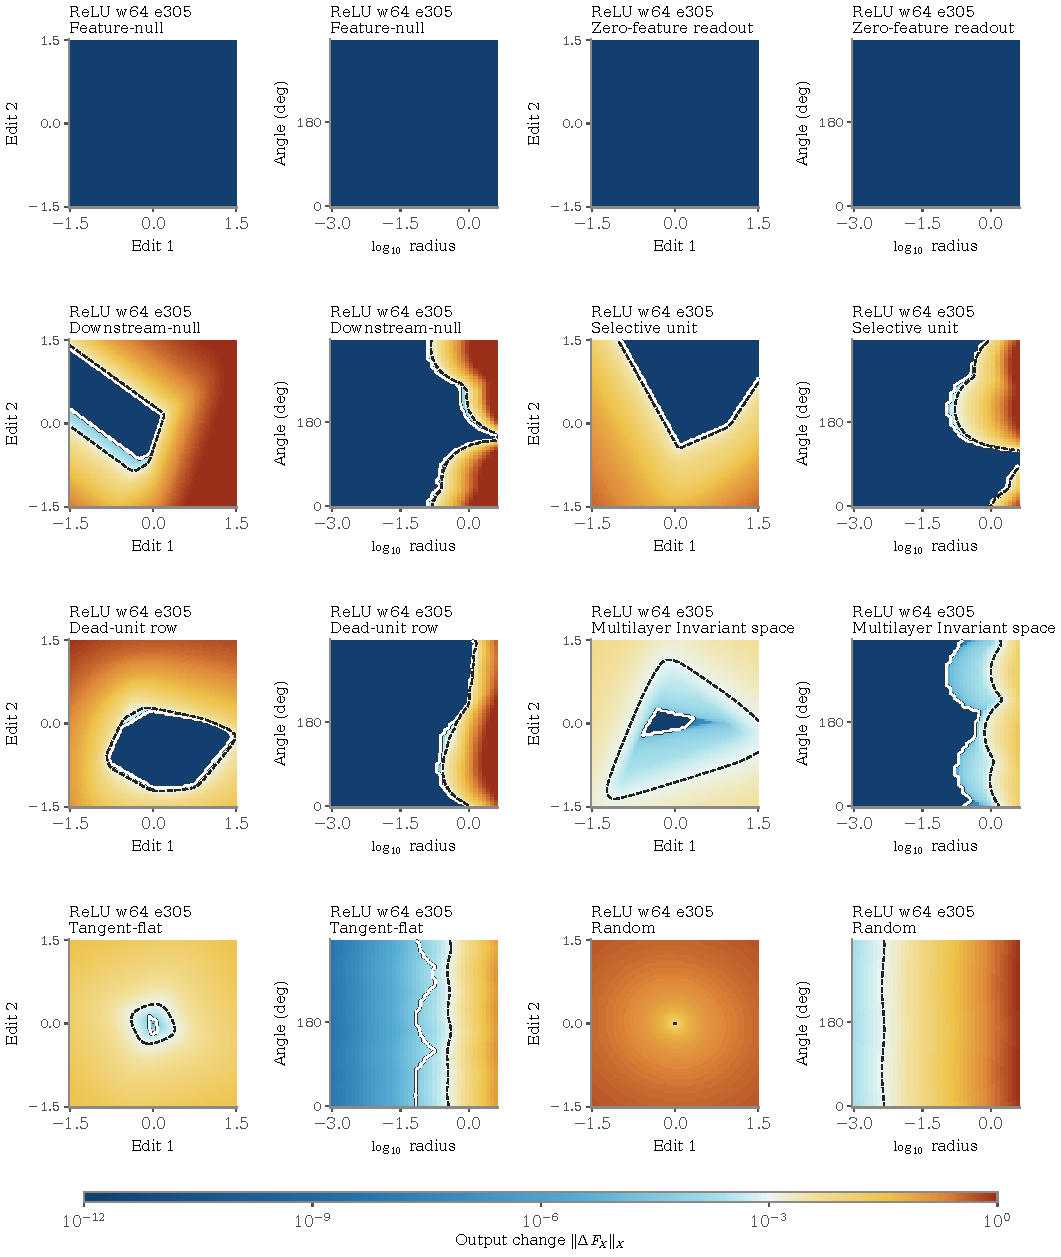
\includegraphics[width=6.367in]{xray_catalogue_1.pdf}
\caption{Ocean x-ray catalog, page 1. All panels use MNIST and seed 0; titles give width (w), hidden depth (d), and checkpoint epoch (e). Adjacent Cartesian and angle--radius panels describe the same two-dimensional parameter plane. The final seven angle--radius panels of the catalog compare selective directions in width and depth sweeps; width sweeps have depth three and depth sweeps have width 128. White contours separate the sampled zero-gate-change region from changed gates, and black dashed contours mark output change $10^{-3}$. All panels share the color scale; values below $10^{-12}$ use its lowest color. See the text for the scope of these sampled views.}\label{fig:xray-catalogue-1}
\end{figure}
\FloatBarrier\begin{figure}[!htbp]\centering
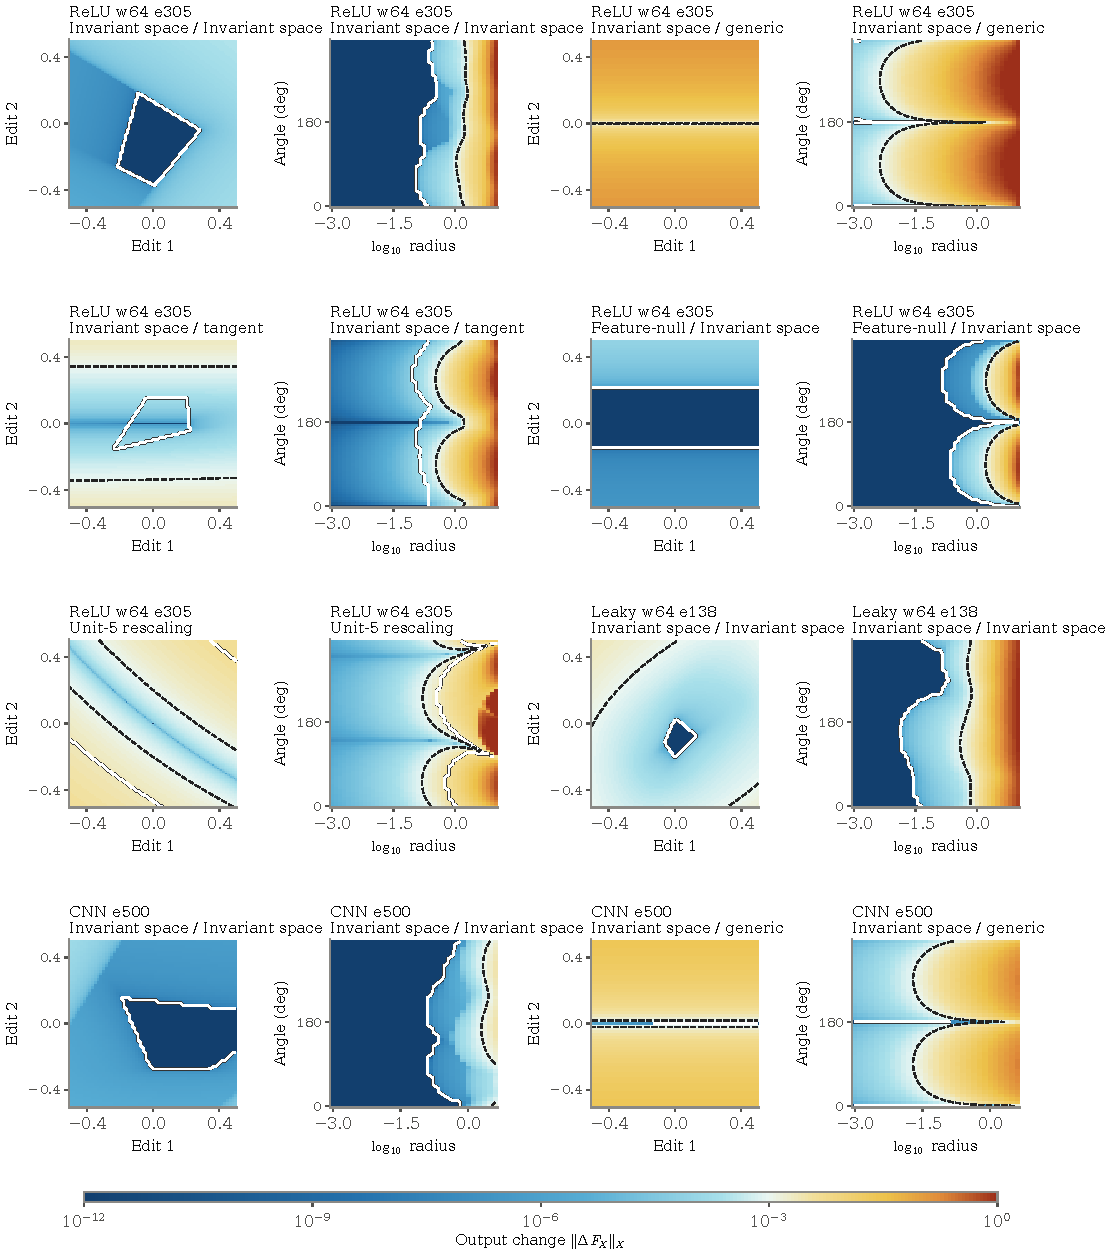
\includegraphics[width=6.662in]{xray_catalogue_2.pdf}
\caption{Ocean x-ray catalog, continued. Conventions and color scale as in Figure~\ref{fig:xray-catalogue-1}.}\label{fig:xray-catalogue-2}
\end{figure}
\FloatBarrier\begin{figure}[!htbp]\centering
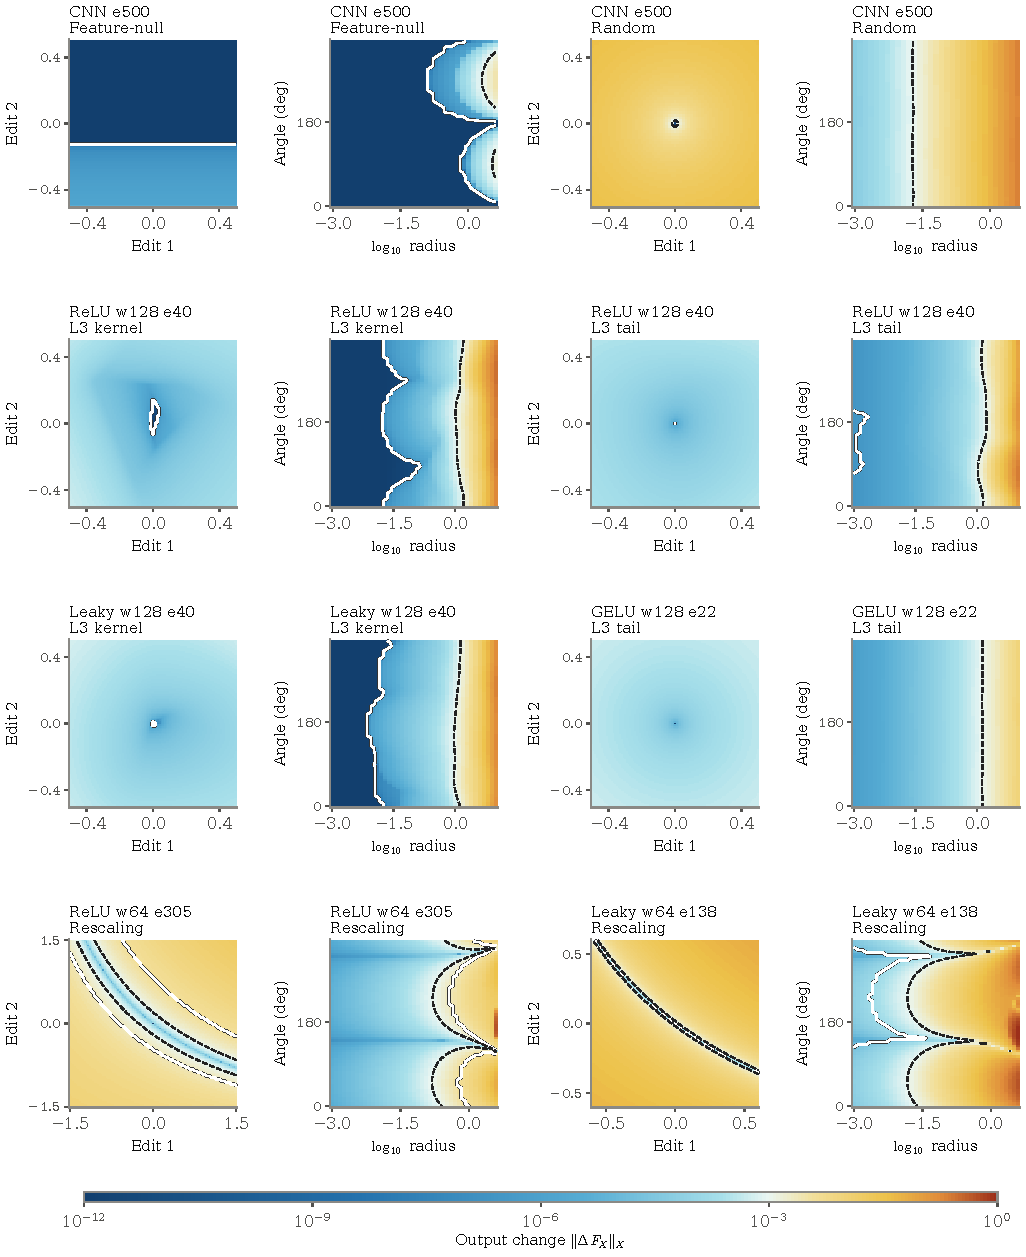
\includegraphics[width=6.156in]{xray_catalogue_3.pdf}
\caption{Ocean x-ray catalog, continued. Conventions and color scale as in Figure~\ref{fig:xray-catalogue-1}.}\label{fig:xray-catalogue-3}
\end{figure}
\FloatBarrier\begin{figure}[!htbp]\centering
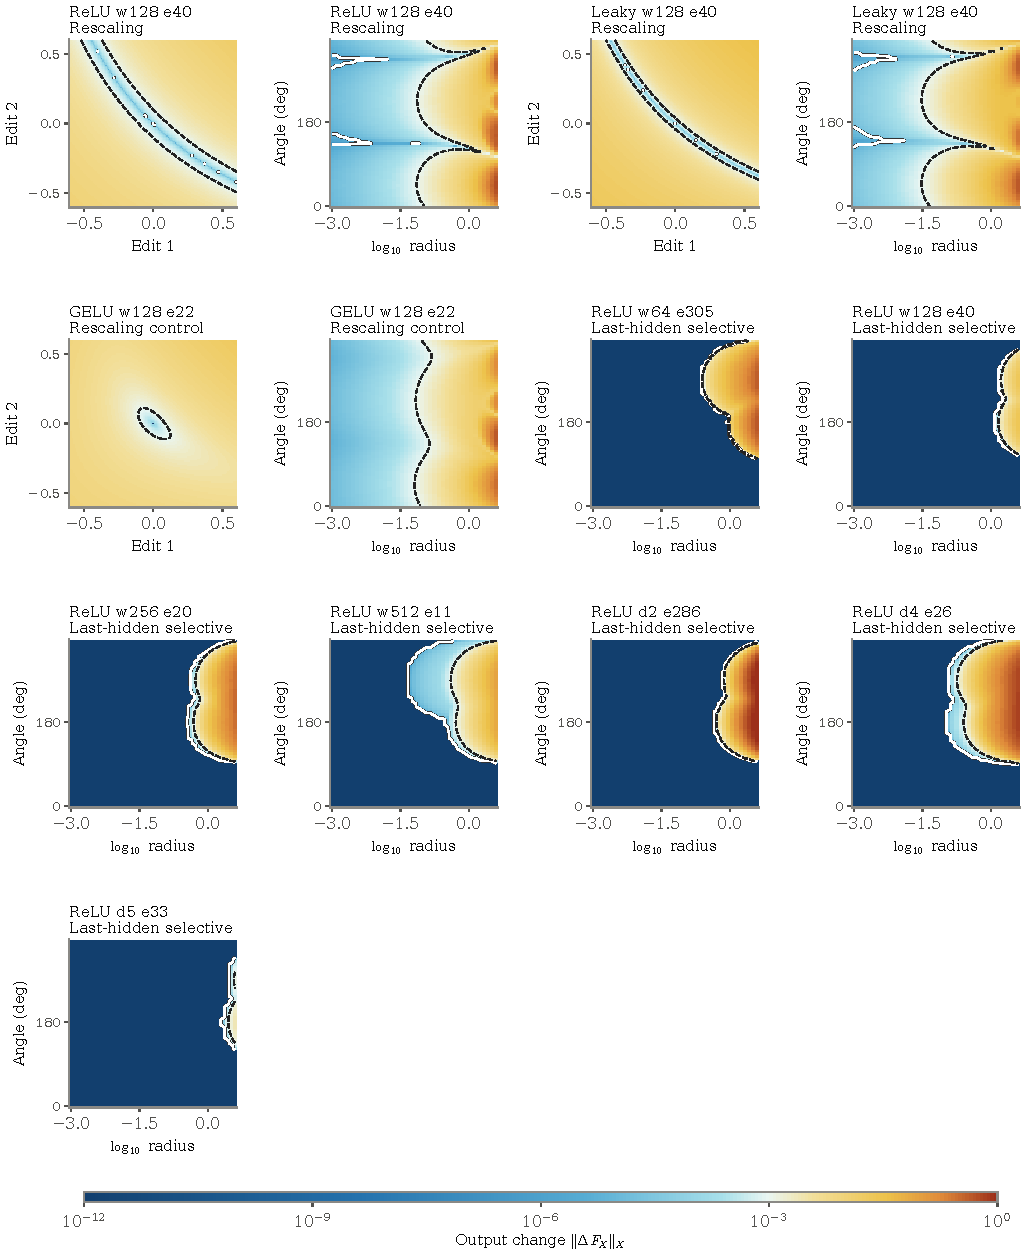
\includegraphics[width=6.156in]{xray_catalogue_4.pdf}
\caption{Ocean x-ray catalog, continued. Conventions and color scale as in Figure~\ref{fig:xray-catalogue-1}.}\label{fig:xray-catalogue-4}
\end{figure}
\FloatBarrier\FloatBarrier
